\chapter{Case Study: RGB Pixel Arrangements}

A pixel is composed of miniature red, green, and blue LEDs. When modeled as a square, there is a red, green, and blue component as well as dark areas. Different phones have different RGB pixel arrangements, and we want to test whether the prefiltering algorithm works regardless of pixel arrangement. We ran the software simulation with the forward method on different pixel arrangements. We consider the scenario with no pixel arrangements, which is the same as a RGB order on an OpenCV image, and a base case of a pixel with simple red, green, and blue bars, in that order. The different devices that we considered are the iPhone \footnote{Link to iPhone pixel: https://www.androidheadlines.com/2013/04/samsung-shows-off-the-new-diamond-pixel-layout-behind-the-s4s-amoled-display.html \cite{android:headlines}} and three generations of Samsung \footnote{Link to Samsung Galaxy S2 pixel: http://www.gsmarena.com/samsung\_galaxy\_note\_ii-review-811p3.php \cite{gsmarena}} \footnote{Link to Samsung Galaxy S3 pixel: https://www.androidheadlines.com/2013/04/samsung-shows-off-the-new-diamond-pixel-layout-behind-the-s4s-amoled-display.html \cite{android:headlines}}  \footnote{Link to Samsung Galaxy S4 pixel: https://www.chipworks.com/ko/node/126 \cite{chipworks}}. We chose a focus at 400 mm, distance of 350 mm, and a screen size of 640x640 pixels. In addition, for the simulation, we compared normalizing by total number of hits and normalizing by the number of hits per color.

\section{Results}

% TODO: rerun no pixel arrangement with pixel size = 78 micrometers
% TODO: rerun pixel arrangement with bug fixed just to see if there is a difference

\begin{figure}
    \centering
    \textbf{No Pixel Arrangements}\par\medskip
    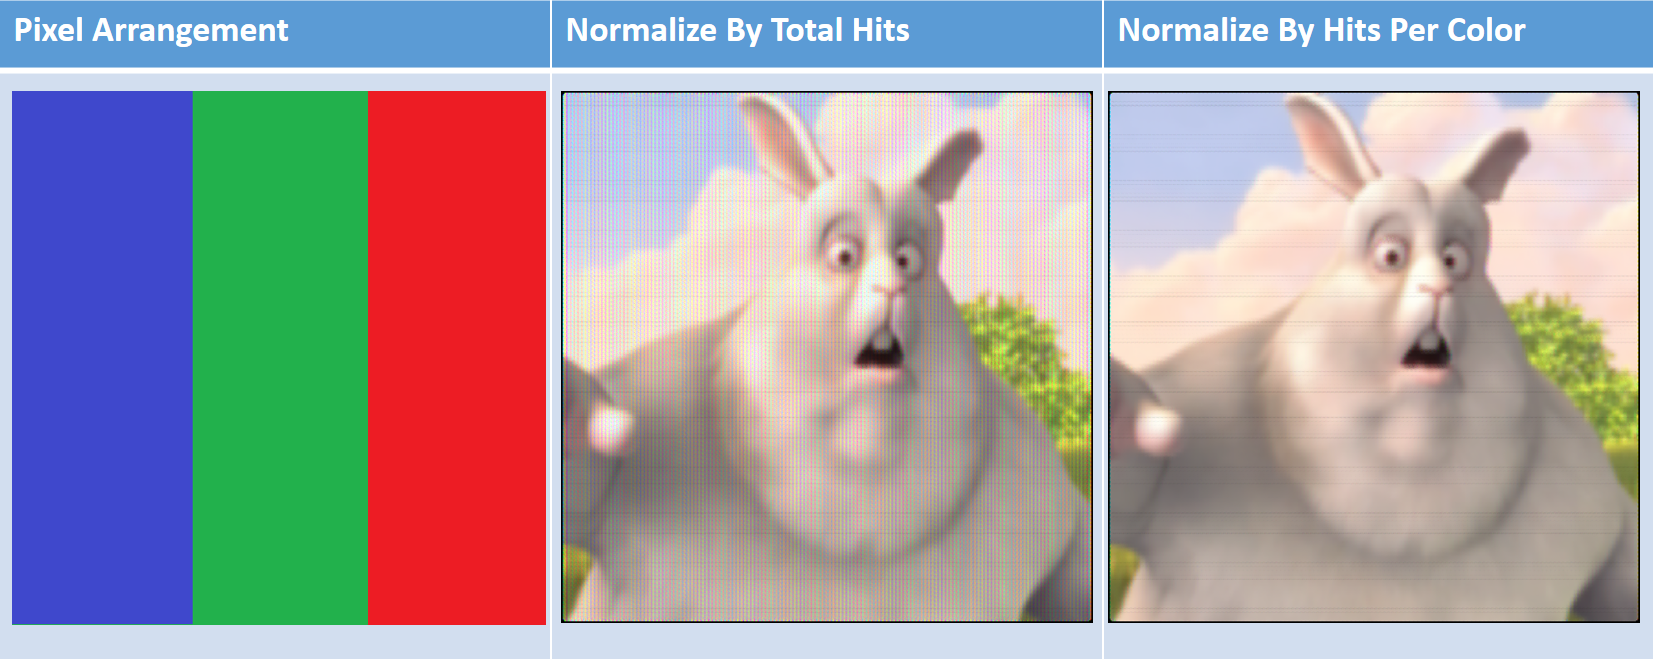
\includegraphics[width=6in]{chapters/chapter7/images/No_Pixel_Arrangement.png}
\end{figure}

\begin{figure}
    \centering
    \textbf{Base Case: RGB Bar}\par\medskip
    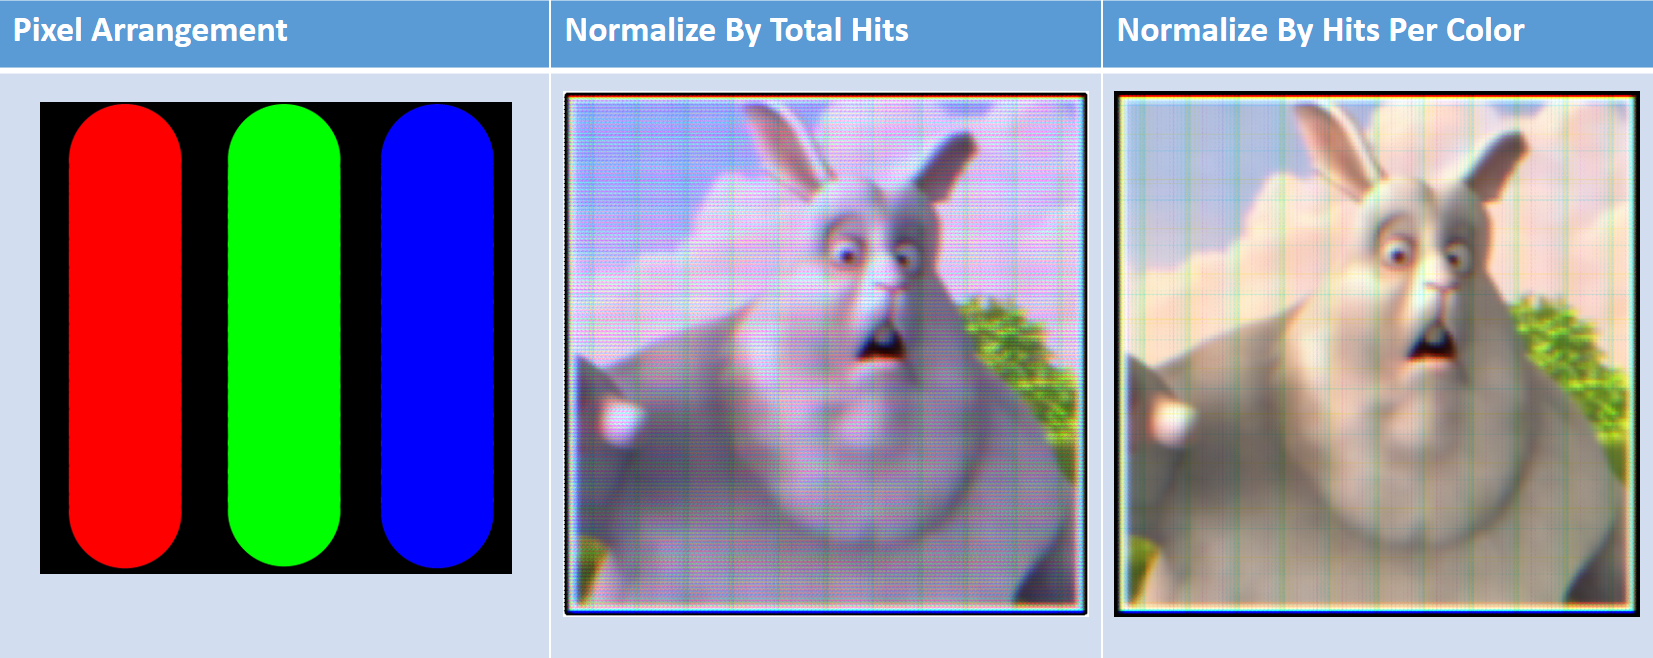
\includegraphics[width=6in]{chapters/chapter7/images/RGB_Bar.png}
\end{figure}

\begin{figure}
    \centering
    \textbf{iPhone}\par\medskip
    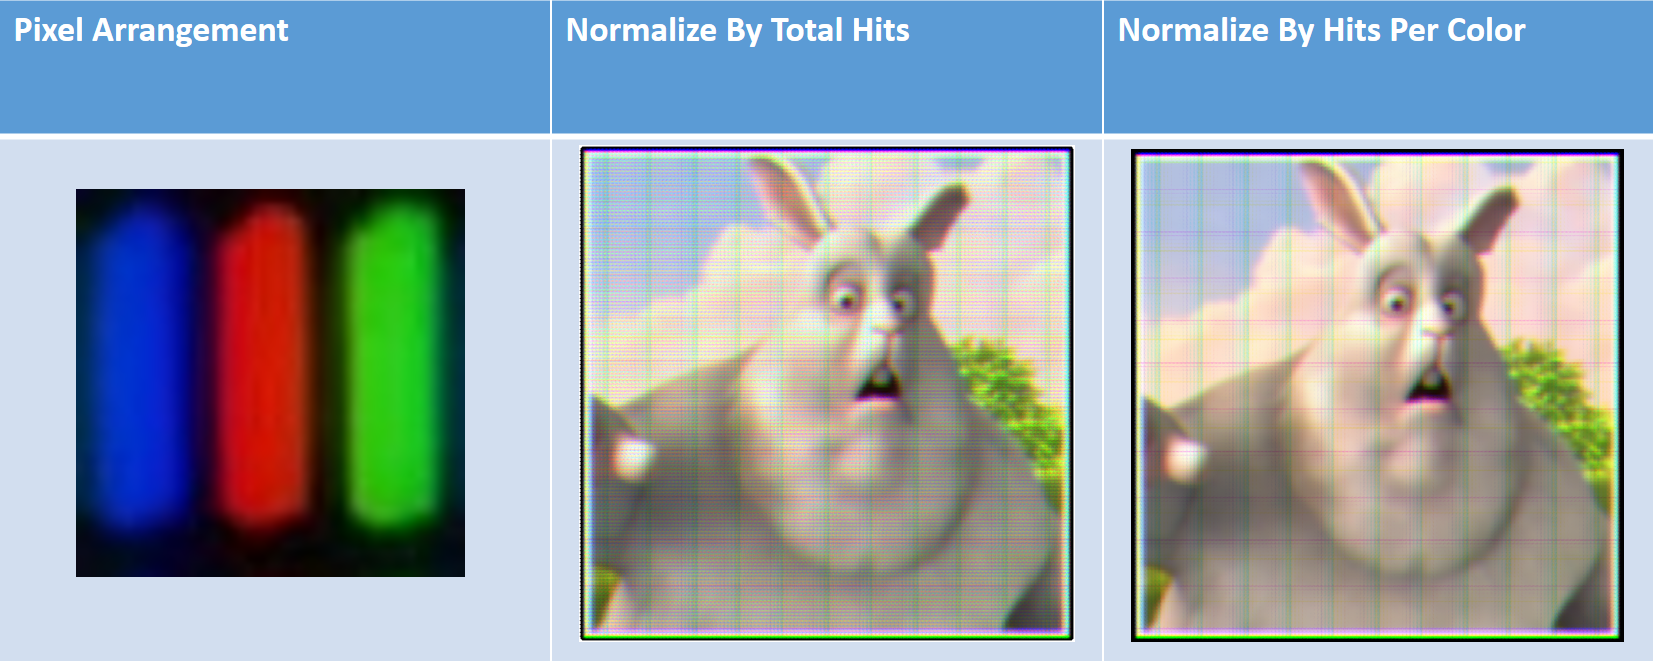
\includegraphics[width=6in]{chapters/chapter7/images/iPhone.png}
\end{figure}

\begin{figure}
    \centering
    \textbf{Samsung Galaxy S2}\par\medskip
    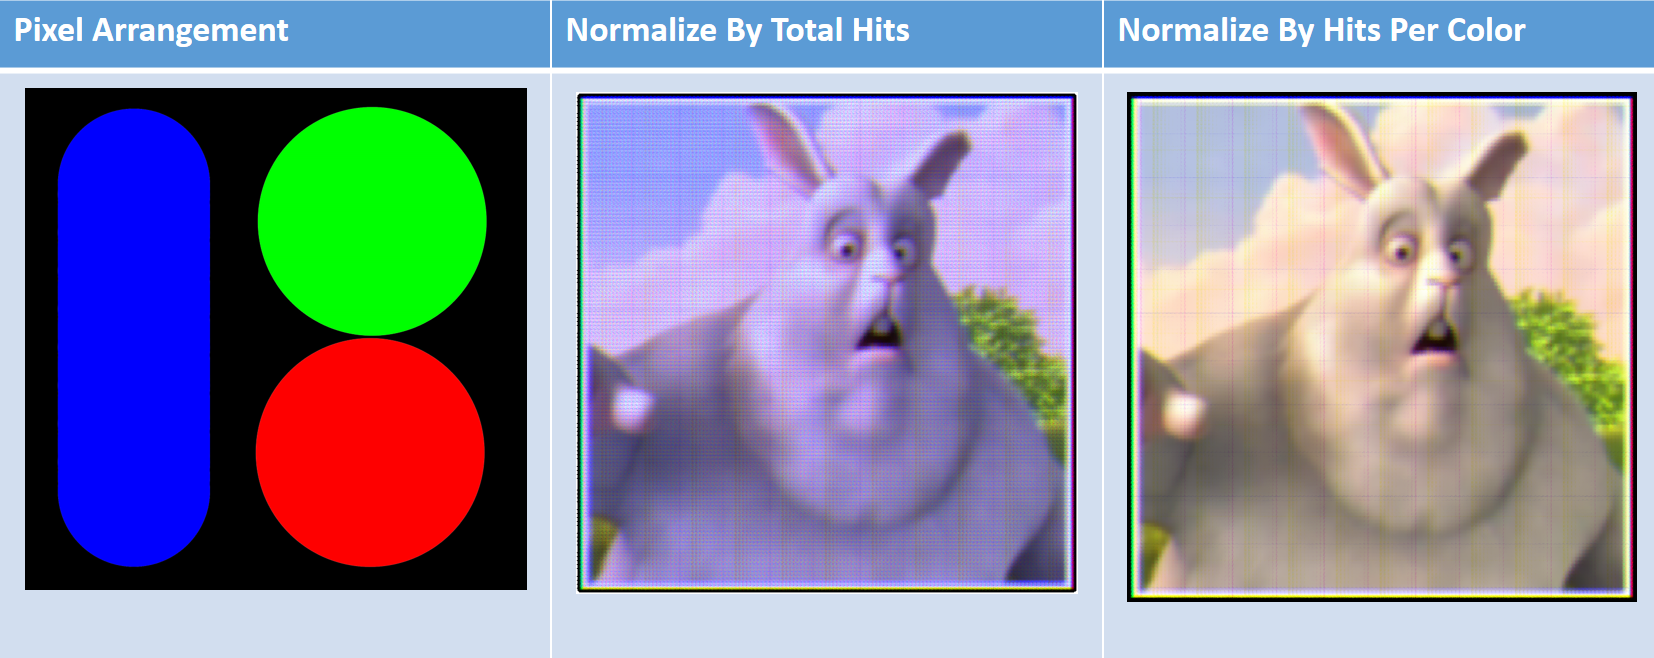
\includegraphics[width=6in]{chapters/chapter7/images/Samsung_Galaxy_S2.png}
\end{figure}

\begin{figure}
    \centering
    \textbf{Samsung Galaxy S3}\par\medskip
    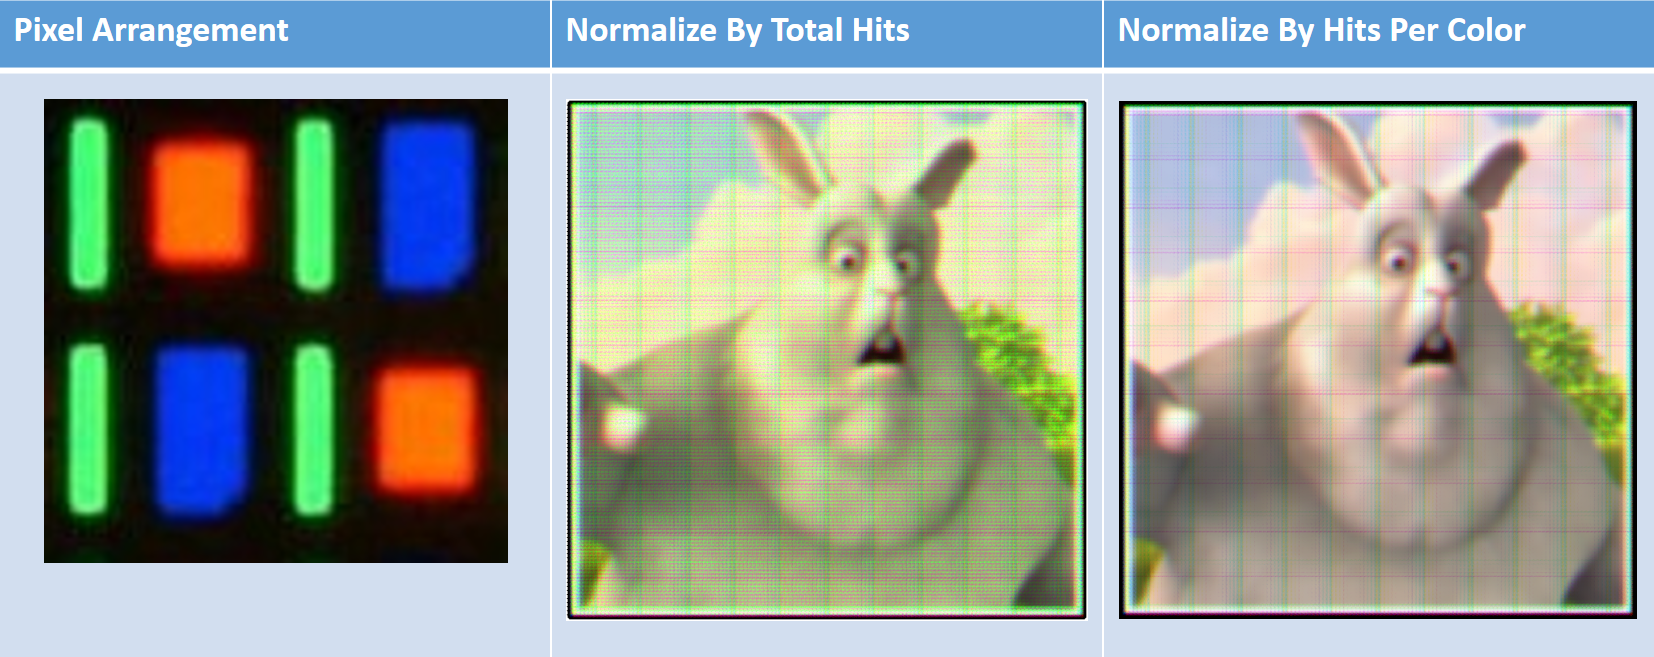
\includegraphics[width=6in]{chapters/chapter7/images/Samsung_Galaxy_S3.png}
\end{figure}

\begin{figure}
    \centering
    \textbf{Samsung Galaxy S4}\par\medskip
    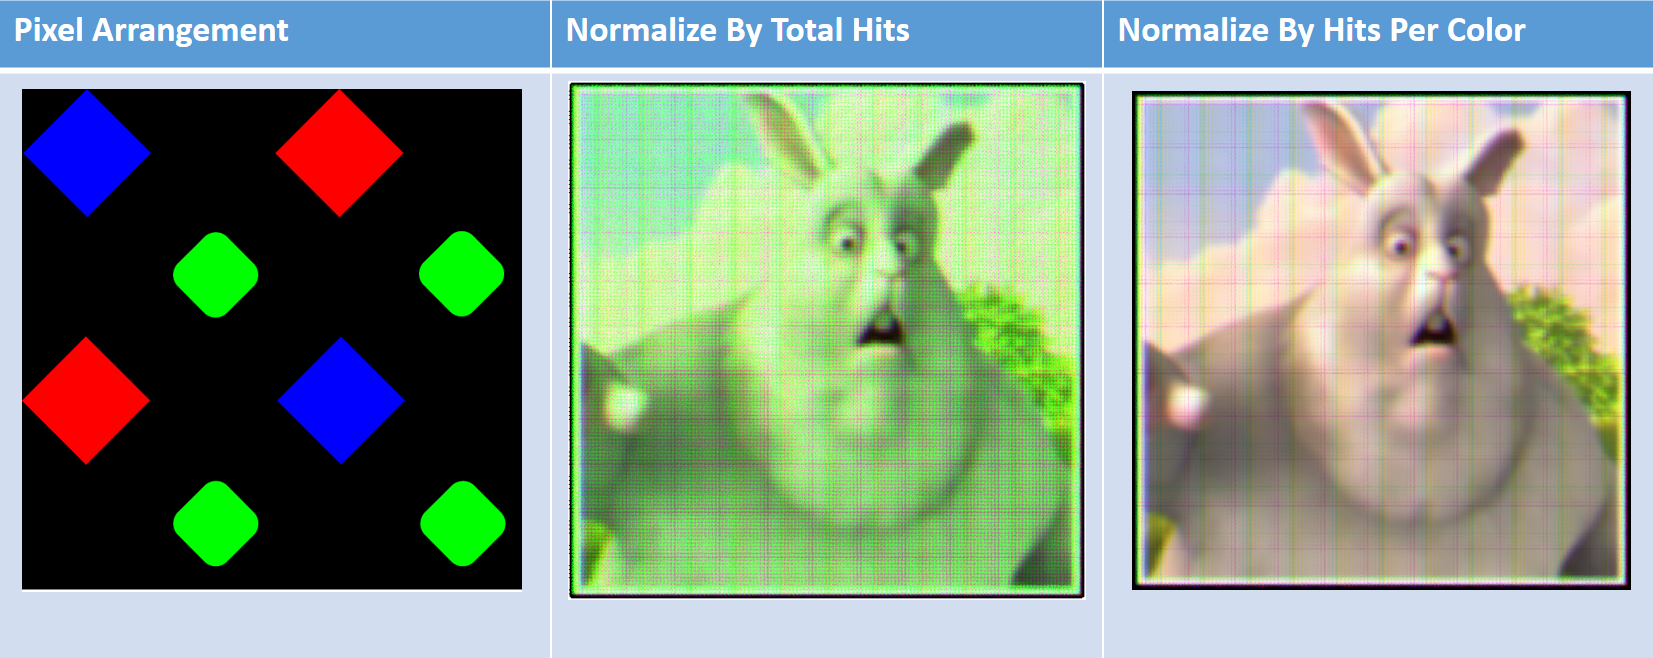
\includegraphics[width=6in]{chapters/chapter7/images/Samsung_Galaxy_S4.png}
\end{figure}

\newpage
\section{Analysis}

The default simulation (OpenCV RGB bars) yields the best results, which is expected. The RGB Bar and the Samsung Galaxy S2 have images that are bright with a blue hue when normalization by the total number of hits is considered. This is expected for the Samsung Galaxy S2 since the the blue LED covers a larger area than the green or red LED, but very unusual for the RGB bar, which has equal red, green, and blue. The iPhone does not have any unique shade, which is expected. The Samsung Galaxy S3 and especially the Samsung Galaxy S4 have a green shade when normalized by the total number of hits, possibly due to a disproportionate amount of green rays as a result of a larger green area on the pixel. All images look very clear when normalized by hits per color and yield a similar grid pattern. The grid pattern is more severe for pixel arrangements with a larger black area as a percentage of total area, which makes sense because more light rays will miss the screen and deviate from the no pixel arrangement case.

% In the future, calculate a percentage of R, G, and B for each pixel arrangement

% In the future, rerun with bug fixed to see if there is any difference

% Also hid the fact that we used 78 micrometer pinhole

% Also missing sources for the pixel arrangements

As expected, the pixel arrangement creates a major impact when we normalize by the total hits because there is a disproportionate amount of red, green, and blue hits when the red, green, and blue components are not equal in area or on different positions of the pixel. However, when we normalize by hits per color, this issue is resolved. The grided pattern may be a result of some pixels on the sensor that have rays traced to unexpected areas on the screen, but it does not interfere much with clear recognition of the bunny.